% !TeX spellcheck = ru_RU-Russian

\documentclass{beamer}
\mode<presentation>
\usetheme{Ilmenau}

\setbeameroption{show notes on second screen}

\author{Василий Генералов \\ VSGeneralov@sberbank.ru}
\title{Machine Learning 101}

\usepackage[utf8]{inputenc}
\usepackage[T1,T2A]{fontenc}
\usepackage{hyperref}
\hypersetup{colorlinks=true,pageanchor=true}
\usepackage{tikz}
\usetikzlibrary{fit}
\usepackage{pgfplots}
\pgfplotsset{compat=newest}

%%% dude wtf
\usepackage{fancyvrb}
\makeatletter
\def\KV@FV@lastline@default{%
  \let\FancyVerbStopNum\m@ne
\let\FancyVerbStopString\relax}
\fvset{lastline}
\makeatother
\usepackage{minted}
%%%

\def \MinSize {22}
\def \TikzScale {0.7}

\newcommand{\mtx}[1]{\boldsymbol{#1}}

\tikzstyle{fcnode}=[
  draw=black,
  rectangle,
  minimum height=2*\MinSize,
  minimum width=1.5*\MinSize
]

\tikzstyle{neuron}=[
  draw=black,
  circle,
  minimum size=\MinSize
]

\begin{document}

\begin{frame}
  \maketitle
\end{frame}

\begin{frame}
  \tableofcontents
\end{frame}

\section{Модель нейрона}

\begin{frame}{\secname : \subsecname}
  \framesubtitle{Сумматор}

  \note{Биологический нейрон реагирует на спайки~--- импульсы,
    приходящие на аксоны, но импульсное поведение сложно моделировать.
    Самой удобной моделью оказался линейный сумматор. Множество $w_i$
  принято называть весами нейрона, а свободный член $b$~--- смещением.}

  \begin{columns}

    \begin{column}{0.5\textwidth}
      $$ y = \sum_{i}^{} w_i \cdot x_i + b $$
    \end{column}

    \begin{column}{0.5\textwidth}
      \begin{center}
        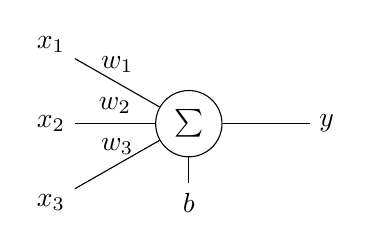
\begin{tikzpicture}
          \def \x {3}
          \def \y {0}
          \def \xOff {1.75}
          \def \yOff {1}

          \node[neuron] (n1) at (\x, \y) {$\sum$};

          % ins
          \node (x1) at (\x - \xOff, \y + \yOff) {$x_1$};
          \node (x2) at (\x - \xOff, \y) {$x_2$};
          \node (x3) at (\x - \xOff, \y - \yOff) {$x_3$};
          \node (b1) at (\x, \y - \yOff) {$b$};

          % out
          \node (y1) at (\x + \xOff, \y) {$y$};

          % connect ins
          \foreach \i in {1,...,3}{
            \draw (x\i) -- (n1) node[midway,above] {$w_\i$};
          }
          \draw (b1) -- (n1);

          % connect out
          \draw (n1) -- (y1);
        \end{tikzpicture}
      \end{center}
    \end{column}

  \end{columns}
\end{frame}

\section{Линейный слой}

\begin{frame}{\secname : \subsecname}
  \framesubtitle{Полносвязный слой, fully connected, linear}
  \begin{columns}

    \begin{column}{0.5\textwidth}
      Здесь и далее используются обозначения, принятые в PyTorch:
      $$
      y = x \cdot \mtx{A}^T + \mtx{b}
      $$
      где $\mtx{A}[O \times I]$~--- матрица обучаемых весов,
      $\mtx{b}[O]$~--- вектор обучаемых смещений,
      подробнее в
      \href{https://docs.pytorch.org/docs/stable/generated/torch.nn.Linear.html}{документации}

    \end{column}

    \begin{column}{0.5\textwidth}
      \begin{center}
        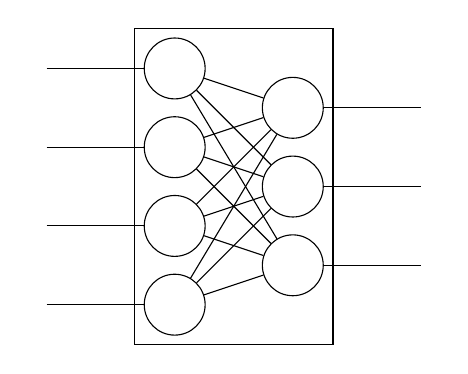
\begin{tikzpicture}
          \def \InSize {3}
          \def \OutSize {2}

          \def \OffX {1.75}

          \def \InX {0}
          \def \InY {-3}
          \def \OffInY {1}

          \def \OutX {1.5}
          \def \OutY {-2.5}
          \def \OffOutY {1}

          \foreach \i in {0,...,\InSize}{
            \def \y {\InY + \i * \OffInY}
            \node[neuron] (n\i) at (\InX, \y) {};
            \node (x\i) at (\InX - \OffX, \y) {};
            \draw (x\i) -- (n\i);
          }

          \foreach \i in {0,...,\OutSize}{
            \def \y {\OutY + \i * \OffOutY}
            \node[neuron] (m\i) at (\OutX, \y) {};
            \node (z\i) at (\OutX + \OffX, \y) {};
            \draw (z\i) -- (m\i);
          }

          \foreach \i in {0,...,\InSize}{
            \foreach \j in {0,...,\OutSize}{
              \draw (n\i) -- (m\j);
            }
          }

          \node[draw, fit=(n0) (n\InSize) (m0) (m\OutSize)] {};
        \end{tikzpicture}
      \end{center}
    \end{column}

  \end{columns}
\end{frame}

\begin{frame}[fragile]{\secname : \subsecname}
  \framesubtitle{Описание модели}
  \inputminted[firstline=19,lastline=25]{python}{linear_regression_1/linear_regression_1.py}
\end{frame}

\begin{frame}{\secname : \subsecname}
  \framesubtitle{Регрессия линейной функции}
  \begin{columns}

    \begin{column}{0.5\textwidth}
      \begin{tikzpicture}[scale=\TikzScale]
        \begin{axis}[title=Результат регрессии,xlabel=$x$,ylabel=$y$,legend
          entries={Исходная функция,Исходная функция + шум,Предсказание модели}]
          \addplot[blue] table[x=X,y=Y,col sep=comma]
          {linear_regression_1/output.csv};
          \addplot[blue,only marks,mark size=1] table[x=X,y=Ynoise,col
          sep=comma] {linear_regression_1/output.csv};
          \addplot[red] table[x=X,y=Ypred,col sep=comma]
          {linear_regression_1/output.csv};
        \end{axis}
      \end{tikzpicture}
    \end{column}

    \begin{column}{0.5\textwidth}
      \begin{tikzpicture}[scale=\TikzScale]
        \begin{axis}[title=Потери,xlabel=Эпоха,ylabel=MSE,legend
          entries={Валидация,Обучение}]
          \addplot[blue] table[col sep=comma]
          {linear_regression_1/test_loss.csv};
          \addplot[red] table[col sep=comma]
          {linear_regression_1/train_loss.csv};
        \end{axis}
      \end{tikzpicture}
    \end{column}

  \end{columns}
\end{frame}

\begin{frame}{\secname : \subsecname}
  \framesubtitle{Регрессия произвольной функции}
  Проведем регрессию $\sin(x)$:

  \begin{columns}
    \begin{column}{0.5\textwidth}
      \begin{tikzpicture}[scale=\TikzScale]
        \begin{axis}[title=Результат регрессии,xlabel={$x$,
            $^{\circ}$},ylabel=$y$,legend
          entries={Исходная функция,Исходная функция + шум,Предсказание модели}]
          \addplot[blue] table[x=X,y=Y,col sep=comma]
          {linear_regression_2/output.csv};
          \addplot[blue,only marks,mark size=1] table[x=X,y=Ynoise,col
          sep=comma] {linear_regression_2/output.csv};
          \addplot[red] table[x=X,y=Ypred,col sep=comma]
          {linear_regression_2/output.csv};
        \end{axis}
      \end{tikzpicture}
    \end{column}

    \begin{column}{0.5\textwidth}
      \begin{tikzpicture}[scale=\TikzScale]
        \begin{axis}[title=Потери,xlabel=Эпоха,ylabel=MSE,ymode=log,legend
          entries={Валидация,Обучение}]
          \addplot[blue] table[col sep=comma]
          {linear_regression_2/test_loss.csv};
          \addplot[red] table[col sep=comma]
          {linear_regression_2/train_loss.csv};
        \end{axis}
      \end{tikzpicture}
    \end{column}
  \end{columns}
\end{frame}

\section{Нелинейность}

\begin{frame}{\secname : \subsecname}
  \framesubtitle{Активация}
  Нелинейность в модель добавляет функция активации

  \begin{columns}

    \begin{column}{0.5\textwidth}

      $$
      y = g\left(\sum_{i}^{} w_i \cdot x_i + b\right)
      $$
      где $g(x)$~--- функция активации (Sigmoid, ReLU, $\tanh$, и т.д.)

    \end{column}

    \begin{column}{0.5\textwidth}
      \begin{center}
        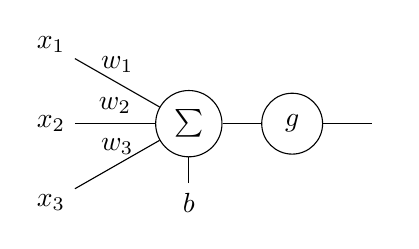
\begin{tikzpicture}
          \def \x {3}
          \def \y {0}
          \def \xOff {1.75}
          \def \yOff {1}

          \node[neuron] (n1) at (\x, \y) {$\sum$};

          \node (x1) at (\x - \xOff, \y + \yOff) {$x_1$};
          \node (x2) at (\x - \xOff, \y) {$x_2$};
          \node (x3) at (\x - \xOff, \y - \yOff) {$x_3$};
          \node (b1) at (\x, \y - \yOff) {$b$};

          \node[neuron] (y1) at (\x + 0.75 * \xOff, \y) {$g$};
          \node (y2) at (\x + 1.4 * \xOff, \y) {};

          \foreach \i in {1,...,3}{
            \draw (x\i) -- (n1) node[midway,above] {$w_\i$};
          }
          \draw (b1) -- (n1);

          \draw (n1) -- (y1);
          \draw (y1) -- (y2);
        \end{tikzpicture}
      \end{center}
      В некоторых источниках сочетание нейрон/линейный слой +
      активация называют <<перцептрон>>
    \end{column}

  \end{columns}
\end{frame}

\begin{frame}{\secname : \subsecname}
  \framesubtitle{Sigmoid, ReLU}

  \begin{columns}

    \begin{column}{0.5\textwidth}
      \begin{tikzpicture}[scale=\TikzScale]
        \begin{axis}[title=Sigmoid,xlabel=$x$,ylabel=$g$,legend
          entries={$\frac{1}{1+\exp^{-x}}$},legend pos=north west]
          \addplot[blue] table[x=X,y=Sigmoid,col sep=comma]
          {activation/output.csv};
        \end{axis}
      \end{tikzpicture}
    \end{column}

    \begin{column}{0.5\textwidth}
      \def \ReLU {$\max(0,x)$}
      \begin{tikzpicture}[scale=\TikzScale]
        \begin{axis}[title=ReLU,xlabel=$x$,ylabel=$g$,legend
          entries={\ReLU},legend pos=north west]
          \addplot[blue] table[x=X,y=ReLU,col sep=comma]
          {activation/output.csv};
        \end{axis}
      \end{tikzpicture}
    \end{column}

  \end{columns}
\end{frame}

\begin{frame}{\secname : \subsecname}
  \framesubtitle{$\tanh$, GELU}

  \begin{columns}

    \begin{column}{0.5\textwidth}
      \begin{tikzpicture}[scale=\TikzScale]
        \begin{axis}[title=Sigmoid,xlabel=$x$,ylabel=$g$,legend
          entries={$\tanh(x)$},legend pos=north west]
          \addplot[blue] table[x=X,y=tanh,col sep=comma]
          {activation/output.csv};
        \end{axis}
      \end{tikzpicture}
    \end{column}

    \begin{column}{0.5\textwidth}
      \begin{tikzpicture}[scale=\TikzScale]
        \begin{axis}[title=GELU,xlabel=$x$,ylabel=$g$,legend
          entries={$x \cdot \Phi(x)$},legend pos=north west]
          \addplot[blue] table[x=X,y=GELU,col sep=comma]
          {activation/output.csv};
        \end{axis}
      \end{tikzpicture}
    \end{column}

  \end{columns}
\end{frame}

\begin{frame}{\secname : \subsecname}
  \framesubtitle{Описание модели}
  \inputminted[firstline=19,lastline=30]{python}{linear_regression_3/linear_regression_3.py}
\end{frame}

\begin{frame}{\secname : \subsecname}
  \framesubtitle{Регрессия произвольной функции}

  \begin{columns}
    \begin{column}{0.5\textwidth}
      \begin{tikzpicture}[scale=\TikzScale]
        \begin{axis}[title=Результат регрессии,xlabel={$x$,
            $^{\circ}$},ylabel=$y$,legend pos=north west,legend
            entries={\tiny{Исходная функция},\tiny{Исходная функция +
          шум},\tiny{Предсказание модели}}]
          \addplot[blue] table[x=X,y=Y,col sep=comma]
          {linear_regression_3/output.csv};
          \addplot[blue,only marks,mark size=1] table[x=X,y=Ynoise,col
          sep=comma] {linear_regression_3/output.csv};
          \addplot[red] table[x=X,y=Ypred,col sep=comma]
          {linear_regression_3/output.csv};
        \end{axis}
      \end{tikzpicture}
    \end{column}

    \begin{column}{0.5\textwidth}
      \begin{tikzpicture}[scale=\TikzScale]
        \begin{axis}[title=Потери,xlabel=Эпоха,ylabel=MSE,legend
          entries={Валидация,Обучение}]
          \addplot[blue] table[col sep=comma]
          {linear_regression_3/test_loss.csv};
          \addplot[red] table[col sep=comma]
          {linear_regression_3/train_loss.csv};
        \end{axis}
      \end{tikzpicture}
    \end{column}
  \end{columns}
\end{frame}

\end{document}
